\documentclass[10pt]{article}
\usepackage[margin=1in]{geometry}
\usepackage{booktabs}
\usepackage{amsmath}
\usepackage{hyperref}
\usepackage{graphicx}

\title{When Plan-Graph Matching Misleads: A Multi-Layer Audit of Tool-Use Plan Evaluation}
\author{Anonymous Authors}
\date{}

\begin{document}
\maketitle

\begin{abstract}
Tool-use plans are commonly scored against one reference graph even though a
task may admit several valid decompositions. Rather than claiming a universally
better metric, we audit when reference matching is informative, when it is
misleading, and what additional evidence is needed. A controlled construct
study crosses 50 symbolic tasks
with seven plan variants (350 plans). In this deliberately balanced design,
exact reference matching rejects 86.7\% of valid non-reference plans. Node F1
has weak rank agreement with deterministic execution (Spearman $\rho=0.188$,
95\% task-cluster bootstrap CI $[0.187,0.192]$), while edge F1 is stronger
($\rho=0.638$, $[0.614,0.661]$). A contract-aware diagnostic, ExecPlanEval,
separates all designed variants (AUROC 1.00), but this is only an internal
construct check because the evaluator and generator share symbolic contracts.

We therefore add external diagnostics rather than treating the controlled
result as open-world validation. Among 360 Qwen3-8B plans for TaskBench and
WorFBench tasks, 99.4\% are valid DAGs, but reference agreement varies sharply
by subset. Two complete blind annotation passes on the fixed run-1 sample agree
on 75.8\% of overall-validity labels ($\kappa=0.536$, 95\% bootstrap CI
$[0.409,0.667]$). A separate record adjudicates all 29 disagreements, producing
72 valid, 21 partially valid, and 27 invalid labels. Against this final layer,
node F1 has AUROC 0.572 ($[0.473,0.672]$) and edge F1 has AUROC 0.458
($[0.362,0.551]$); both intervals include chance. Separately, a reactive
Qwen3-8B policy completes 35 of 120 ALFWorld tasks despite selecting only
admissible commands. In a matched 30-task test, single-shot plans generated
from the initial state score 0.934 on our pre-execution checks yet complete
0/30 tasks, versus 8/30 for reactive execution ($p=0.0078$, exact McNemar
test). On the 40 TaskBench tasks with benchmark-supplied tool
input/output types, a reference-free typed-contract diagnostic reaches AUROC
0.631 ($[0.470,0.809]$). Together, the studies expose three distinct failure
modes: multiplicity in valid plans, benchmark-dependent representation, and
the gap between locally legal actions and completed tasks. They do not establish
external superiority for ExecPlanEval: natural tasks lack the required
contracts, and the annotation files do not authenticate contributor identity or
independence. The main contribution is therefore an evidence hierarchy and a
set of boundary conditions for plan evaluation, not a claim that one score
should replace all existing metrics.
An additional 120-plan Gemma3-1B sensitivity run shows substantially lower DAG
and catalog validity, but confounds family, scale, and decoding constraint.
\end{abstract}

\noindent\textbf{Keywords:} language agents; tool planning; task
decomposition; graph evaluation; execution-grounded evaluation

\section{Introduction}
Language-model agents increasingly handle complex tasks by choosing tools,
filling in their arguments, and arranging calls into dependency-aware plans.
Benchmarks such as TaskBench~\cite{shen2024taskbench} and
WorFBench~\cite{qiao2025worfbench} have made these capabilities measurable by
comparing predicted workflows with reference structures.
That style of evaluation makes a strong, often implicit assumption: structural
agreement with the reference stands in for actual plan validity. It becomes
hard to defend when independent steps can be reordered, two tools can achieve
the same subgoal, or an extra harmless check makes a plan more robust.

We examine the gap between looking like the reference and actually working---a
distinction that becomes more important as agent plans grow longer and less
canonical. Specifically, we ask whether node and edge matching rank candidate
plans correctly, how often these metrics reject valid alternatives, and
whether outcome-grounded signals align more closely with verified validity.
Our goal is methodological diagnosis: to identify which conclusions each
evidence source can and cannot support. The paper makes four contributions:

\begin{itemize}
  \item We construct a controlled benchmark that pairs valid alternative plans
  with diagnostically targeted invalid perturbations.
  \item We use ExecPlanEval as a modular diagnostic that separates goal
  coverage, dependency validity, executability, and final-state success; we do
  not treat its controlled-benchmark performance as external superiority.
  \item We provide correlation, confounding, and error analyses that show how
  metric conclusions change across task structure, benchmark representation,
  annotation source, and execution protocol.
  \item We add two external checks: 480 naturally generated plans from
  TaskBench and WorFBench, and 120 live ALFWorld executions with complete
  action--observation trajectories. For 40 TaskBench tasks, we additionally
  evaluate tool membership and edge compatibility against independently
  supplied input/output types. We also release two raw AI-assisted blind
  annotation runs, two completed paired blind annotation workbooks, and a
  separate adjudication layer covering all 29 disagreements. We preserve both
  source passes rather than silently converting either into a gold standard.
  A matched 30-task ALFWorld experiment additionally freezes the entire action
  sequence before execution, separating plan generation from feedback-driven
  control.
\end{itemize}

Three audit questions guide the analysis. \textbf{AQ1} asks when a single
reference graph rejects operationally valid alternatives. \textbf{AQ2} asks
which apparent metric advantages survive changes in benchmark representation,
annotation source, and model. \textbf{AQ3} asks what static checks fail to
capture once plans interact with a partially observable environment. The
controlled experiment answers AQ1 under explicit contracts; natural plans and
annotation address AQ2 descriptively; typed contracts and ALFWorld address AQ3.
Keeping these evidence levels separate is part of the method. None estimates a
general open-world accuracy for ExecPlanEval.

\section{Related Work}
\subsection{Tool-Using Language Agents}
ReAct~\cite{yao2023react} interleaves language-model reasoning, actions, and
environment observations. It has become a common interaction pattern for
tool-using agents. Toolformer~\cite{schick2023toolformer} takes a
self-supervised approach to learning tool use, whereas ToolLLM~\cite{qin2023toolllm},
ToolAlpaca~\cite{tang2023toolalpaca}, and Gorilla~\cite{patil2023gorilla}
develop data, training, and retrieval strategies for broader API use.
RestGPT~\cite{song2023restgpt} explicitly combines coarse-to-fine planning with
real RESTful APIs. API-Bank~\cite{li2023apibank} evaluates planning, tool
retrieval, and API calling in an executable environment, while the Berkeley
Function-Calling Leaderboard~\cite{yan2024bfcl} provides broad function-call
accuracy tests. Taken together, this literature suggests that a textual plan
is only part of the object being evaluated. What happens when the plan is run
matters just as much.

\subsection{Agent Planning Benchmarks}
TaskBench~\cite{shen2024taskbench} represents automation plans as tool graphs
and reports node and edge F1 alongside parameter metrics. WorFBench
~\cite{qiao2025worfbench} broadens workflow generation to diverse scenarios and
uses subsequence and subgraph matching. FlowBench~\cite{xiao2024flowbench}
instead evaluates whether agents can follow workflow knowledge expressed as
text, code, or flowcharts. PlanBench~\cite{valmeekam2024planbench} uses formal
planning domains to test plan generation and reasoning about change, whereas
TravelPlanner~\cite{xie2024travelplanner} evaluates constraint-rich plans in a
realistic sandbox. UltraTool~\cite{huang2024ultratool},
AppBench~\cite{wang2024appbench}, CToolEval~\cite{guo2024ctooleval}, and
PlanningArena~\cite{zheng2025planningarena} extend evaluation to complex tool
creation, cross-application API dependencies, Chinese application scenarios,
and modular planning. StableToolBench~\cite{guo2024stabletoolbench} addresses
API and evaluator instability, RoTBench~\cite{ye2024rotbench} introduces
controlled tool noise, and ToolEyes~\cite{ye2025tooleyes} separates planning,
selection, formatting, and answer organization. Despite their different
settings, many of these benchmarks share an assumption: similarity to one
annotated graph is treated as a good proxy for plan validity. That assumption
is the focus of our study.

Formal-planning work offers a useful counterpoint. Beyond PlanBench, controlled
experiments show that autonomous LLM plans often fail when checked by an
external executor~\cite{valmeekam2023critical}. AutoPlanBench
~\cite{stein2023autoplanbench} automatically translates PDDL domains into
natural-language planning tests, while LLM+P~\cite{liu2023llmp} delegates
sound plan synthesis to a classical planner. These results motivate our use of
explicit preconditions, effects, and executable verification rather than
surface plausibility alone.

\subsection{Agent Evaluation}
Reference matching is deterministic, inexpensive, and easy to reproduce. Its
weakness is subtler: one annotated realization is allowed to stand in for the
whole set of plans that could satisfy the goal. Model-based judges can compare
meaning rather than exact structure, but they bring their own biases and can
miss hard execution constraints. Running the plan gives more direct evidence,
although doing so may be costly or unsafe in an open environment. ExecPlanEval
therefore treats these signals as complementary. Its components remain
visible, and it uses deterministic execution wherever a verifier is available.

Broader agent benchmarks emphasize the same need for environment-grounded
measurement. AgentBench~\cite{liu2023agentbench} spans multiple interactive
environments; AgentBoard~\cite{ma2024agentboard} adds fine-grained progress
tracking; GAIA~\cite{mialon2024gaia} tests general assistants on questions that
require tools; and WebArena~\cite{zhou2024webarena} evaluates functional task
completion on reproducible websites. In text generation, multi-reference
studies likewise show that limited references can depress agreement with human
judgments~\cite{gupta2019multireference,tang2024divref,zeng2024multireference}.
Our setting transfers that multiplicity concern from surface realizations to
executable plan graphs, where semantic equivalence can be checked through tool
contracts and state transitions.

Stateful evaluation is particularly close to the motivation behind our work.
ToolSandbox~\cite{lu2025toolsandbox} scores intermediate and final milestones
over interactive trajectories, and $\tau$-bench~\cite{yao2025taubench} compares
the final database state with an annotated goal while measuring reliability
over repeated trials. ToolEmu~\cite{ruan2024toolemu} uses an LM-emulated sandbox
to examine risky tool behavior. Unlike these open-ended environments, our
controlled study gives up some realism on purpose, allowing us to isolate the
effect of alternative but valid graph structures.

\section{Problem Formulation}
We define a task by an initial state $s_0$, a goal predicate $g$, and a tool
set $\mathcal{T}$. A candidate plan $P=(V,E)$ is a directed acyclic graph:
its nodes are parameterized tool calls, and its edges represent data or
temporal dependencies. We call a plan valid when some allowed topological
execution starts from $s_0$, respects the hard constraints, and ends in a
state satisfying $g$. A plan need not resemble the reference structurally to
meet this definition.

Let $R$ denote the annotated reference and $\mathcal{V}(s_0,g,\mathcal{T})$
the set of plans valid for the task. Reference matching estimates similarity
to the singleton $\{R\}$, whereas operational evaluation asks whether
$P\in\mathcal{V}$. The two questions coincide only in the special case where
the reference is the unique valid plan and the graph representation captures
every constraint.
Tool equivalence violates uniqueness; omitted semantic dependencies violate
representation completeness. This distinction motivates both our candidate
transformations and the component scores below.

For the structural baselines, node precision and recall compare multisets of
tool labels; edge precision and recall compare ordered pairs of endpoint tool
labels. For either item type $z$, $F1_z=2p_zr_z/(p_z+r_z)$, with the usual
zero convention. This formulation mirrors common graph-matching practice while
remaining invariant to arbitrary node identifiers.

\section{A Contract-Aware Diagnostic: ExecPlanEval}
\subsection{Goal Coverage}
Goal coverage asks how much of the requested goal is true in the final state.
In the controlled symbolic benchmark, every predicate is deterministic and directly
observable. A full benchmark would replace these symbolic predicates with
task-specific verifiers.

Formally, if $G$ is the required predicate set and $s_P$ is the terminal state,
$G(P)=|G\cap s_P|/|G|$. The executor reports zero for an empty or malformed
plan unless the initial state already satisfies the goal.

\subsection{Dependency Validation}
Dependency validation examines each tool-call precondition that is not already
true initially. It asks whether some ancestor of the consumer node produces
that precondition. The score is the proportion of these checks that pass.
Independent nodes do not need an artificial order, so a harmless serialization
edge does not make the plan less valid.

For a node $v$, let $\mathrm{pre}(v)$ be its preconditions and let
$\mathrm{anc}(v)$ be its graph ancestors. A non-initial precondition is
supported if some ancestor produces it. Dependency validity $D(P)$ is the
fraction of supported checks. Cyclic graphs are rejected because no valid
topological execution exists.

\subsection{Schema Executability and Outcome Verification}
The implemented executability component is static. It checks graph integrity,
acyclicity, tool membership, and whether each node's declared
precondition/effect schema matches the catalog. It does not award credit for the
fraction of nodes completed before failure. Dynamic behavior is represented
separately by terminal goal coverage and binary outcome success: outcome is one
only when every required goal predicate holds after execution. This distinction
matters because a well-formed plan may execute several calls and still miss the
user's goal, while partial progress is task-dependent and requires a separately
specified utility function.

\subsection{Score Calibration}
\begin{equation}
S(P)=w_gG(P)+w_dD(P)+w_xX_{static}(P)+w_oO(P).
\end{equation}
We fixed the component definitions and equal weights before looking at the
controlled-test results. Any learned calibration should instead be fitted on a
separate validation partition and then frozen before final evaluation.

For the controlled benchmark, we use equal weights and fit no parameters. We also report a
strictly static variant based only on dependency validity and schema-level
executability. It checks tool membership, declared contracts, graph integrity,
and acyclicity without invoking the symbolic executor. This separation prevents
the comparison from reusing the final outcome label that it is supposed to
predict.

The implemented controlled scores are therefore
\begin{equation}
S_{static}(P)=\tfrac{1}{2}\left[D(P)+X_{static}(P)\right],\qquad
S_{full}(P)=\tfrac{1}{4}\left[G(P)+D(P)+X_{static}(P)+O(P)\right].
\end{equation}
Here, $X_{static}$ is the fraction of nodes whose identifiers, tool names, and
declared precondition/effect schemas pass catalog validation, with malformed or
cyclic graphs assigned zero. The individual components are always retained, so the aggregate does not hide
why a plan failed. In deployment, hard safety constraints should override the
weighted score; high values elsewhere must not compensate for a safety breach.

\section{Benchmark Construction}
We built the benchmark to study plan multiplicity without mixing in unrelated
agent errors. It uses ten domain labels (travel, weather, shopping,
media, document processing, meetings, finance, support, research, and
security) crossed with five graph topologies: a four-node chain, a four-node
diamond, a five-node fork--join graph, a six-node double diamond, and a
six-node chain. The resulting 50 tasks use symbolic preconditions and effects,
so validity and final-state success can be verified exactly. The labels do not
create independent domain dynamics: the five topology templates are the
conservative unit of statistical resampling.

Each task starts with one reference plan and has six controlled variants. Three
remain valid:
(i) adding a serialization constraint between otherwise independent nodes,
(ii) substituting a tool with an equivalent tool that has identical
preconditions and effects, and (iii) adding a harmless audit step after goal
completion. Three are invalid: removing a required producer, reversing a
required dependency, and replacing a required tool with an unavailable tool.
With the references included, the benchmark contains 350 candidate plans.
Generation is deterministic. Executable assertions also compare every designed
validity label against the symbolic executor, which guards against a variant
quietly violating its intended category.

The three valid transformations capture different reasons why correct plans
may look different. Serialization changes scheduling freedom and nothing else.
Equivalent substitution changes the tool label but preserves its precondition
and effect contract. Audit insertion adds a post-goal node whose precondition
is already available and whose effect is not required. The invalid cases are
equally targeted. Removing a producer leaves a consumer unsupported; reversing
a required edge prevents a required producer from becoming causally available;
and wrong-tool replacement introduces an unavailable action with an
unsatisfied sentinel precondition. Every topology-domain pair contributes one
candidate of each variant, so the aggregate comparison is not driven by a more
frequent variant.

This construction gives us exact counterfactual control, but there is a clear
trade-off. It does not model ambiguous natural-language goals, stochastic APIs,
permissions, or irreversible effects. We therefore keep the controlled
benchmark conceptually separate from the external validation reported below.

\subsection{External Natural-Plan Sample}
To test whether the pipeline extends beyond designed perturbations, we sampled
20 tasks from each of six public subsets: WikiHow, ALFWorld, and WebShop from
WorFBench, and DailyLife APIs, multimedia, and Hugging Face from TaskBench.
Sampling used seed 20260826 and round-robin allocation across the available
topology labels (or reference-plan lengths when topology labels were absent),
with uniform random selection within each stratum.
Qwen3-8B generated three plans per task, giving 360 outputs. The model saw the
natural-language instruction and available actions, but never the reference
graph. Generation used temperature 0.2, run-index seeds 1--3, a 900-token
budget, and no hidden reasoning. Raw output and parse failures were retained;
there was no retry or structural repair.

As a model-sensitivity diagnostic, we generated one additional plan for every
task with Gemma3-1B. Because an unconstrained pilot produced malformed
near-JSON, this run requested Ollama's JSON-constrained decoding; failures were
still retained without retry or semantic repair. We compare it with run 1 of
Qwen3-8B using paired task-level differences and 2,000 bootstrap resamples.
This is not a controlled family comparison: model family, parameter count, and
decoding constraint all differ. It tests whether conclusions about the pipeline
can be assumed to transfer unchanged to a much smaller non-Qwen model.

We report parse rate, DAG validity, catalog validity, node and edge F1, a fuzzy
node-label F1, and within-task Jaccard stability across runs. These are
descriptive reference-agreement diagnostics, not execution-success measures.
In particular, a low F1 score may reflect different action granularity or
label vocabulary rather than an invalid plan.

For an exploratory semantic check, Qwen3-4B and Qwen3-8B independently labeled
the fixed run-1 plan for all 120 tasks. Both received the same codebook and saw
only the instruction, candidate graph, benchmark, and subset. Model identity,
automatic scores, and reference plans were withheld from the annotation prompt.
Decoding was deterministic and schema-constrained. We report raw agreement and
unweighted Cohen's $\kappa$ with 2,000 task-level bootstrap resamples. A later
rubric audit produced one analysis label per task but did not overwrite either
raw annotation. This protocol is AI-assisted annotation, not independent human
validation: both annotators belong to the Qwen3 family, and Qwen3-8B also
generated the candidate plans.
The schema constrained field values but did not force logical consistency
between fields; consequently, component-level agreement is reported on the raw
outputs as a diagnostic rather than as adjudicated ground truth.
For a confounding check, we encoded audited labels ordinally
(invalid$=0$, partial$=1$, valid$=2$), computed task-bootstrap intervals, and
removed between-subset rank shifts by centering score and label ranks within
each of the six subsets. We compare exact node F1, edge F1, fuzzy node F1, a
simple node--edge overlap average, and catalog validity. Because these outcomes
remain AI-assisted labels, all such analyses are exploratory.

Separately, we prepared two English-language blind workbooks for the same
fixed run-1 sample. Each contained the instruction, candidate plan, benchmark,
and subset, but excluded model identity, automatic scores, and the reference
graph. The codebook required one label for overall validity, tool selection,
dependency validity, executability, goal completion, alternative validity, and
primary error type, plus a free-text rationale. Both returned workbooks contain
all 120 rows and no missing required fields. We report unweighted Cohen's
$\kappa$ and observed agreement with 2,000 paired task-bootstrap resamples
(seed 20260827). We refer to A and B only as paired annotation passes because
workbook contents do not independently establish that two distinct people
completed them without consultation. Raw passes are never overwritten. For the
final analysis layer, labels shared by A and B are retained, while a separately
submitted adjudication record supplies all seven categorical fields for every
case with at least one disagreement. We require an exact match between the
adjudication IDs and the computed disagreement set, valid codebook values, a
rationale, an adjudicator identifier, and a completion date. This produces one
complete label per task without modifying either source workbook. File contents
alone do not verify the adjudicator's identity or independence, so we call this
an adjudicated label set rather than certified independent human ground truth.
We encode overall validity ordinally (invalid$=0$, partial$=1$, valid$=2$) for
Spearman correlation and binarize valid versus partial/invalid for AUROC. Both
use 2,000 fixed-seed task bootstrap resamples; within-subset centered rank
correlation is also reported to expose benchmark confounding.

\subsection{Typed-Contract External Diagnostic}
The natural sample cannot support a complete external ExecPlanEval score:
WorFBench does not expose machine-readable tool contracts, DailyLife APIs lacks
output types, candidate plans omit argument bindings, and no common executor is
available. Inferring contracts from gold edges would reintroduce the reference
anchoring that the study is intended to test. We therefore restrict a
reference-free contract diagnostic to the 40 run-1 TaskBench Multimedia and
Hugging Face plans. Their benchmark-provided \texttt{tool\_desc.json} files list
tool identifiers and input/output types independently of our generated plans.

After normalized exact tool-name matching, catalog validity is the fraction of
candidate nodes found in the supplied catalog. For each predicted edge, type
compatibility is one when the source output-type set intersects the target
input-type set; the edge score is the mean of these checks, with an empty edge
set assigned one. The typed-contract diagnostic averages graph validity,
catalog validity, and edge-type compatibility. It uses neither the reference
graph nor the adjudicated component labels. Overall-validity labels are used
only as the external outcome. We report Spearman correlation and valid-versus-
other AUROC with 2,000 task bootstrap resamples. This diagnostic can detect
unknown tools and type-incompatible edges, but not missing dependencies,
incorrect arguments, goal completion, or execution failure; it is therefore an
external component test, not the complete ExecPlanEval score.

\section{Experimental Setup}
The primary comparison covers node F1, edge F1, and the static ExecPlanEval
score. The post-execution full score is reported descriptively but excluded
from predictive correlation and AUROC because it contains the outcome itself.
Deterministic execution success is the primary dependent variable. We use
Spearman rank correlation and AUROC to
measure how well the scores separate valid and invalid plans. The reported
95\% percentile confidence intervals come from 2,000 non-parametric cluster
bootstrap resamples of the 50 tasks with a fixed seed; all seven variants of a
task are sampled together. Topology is treated as a fixed design factor rather
than as the sampling unit. Under strict matching, a plan is accepted only
when both node F1 and edge F1 are exactly one.

All controlled experiments run in Python with NetworkX. At each step, the
symbolic executor selects lexicographically among actions whose graph
predecessors have completed and whose preconditions hold; it fails only when no
remaining action is enabled. The static score gives equal weight to dependency
validity and schema-level executability. The full score weights goal coverage,
dependency validity, executability, and outcome success equally. None of these
weights is fitted on the evaluation data. We additionally report dependency-only
and static-executability-only ablations.
We also sweep the static dependency weight from 0 to 1 in increments of 0.05,
assigning the remaining weight to schema-level executability. This is a
sensitivity analysis, not weight selection: the controlled data are not an
appropriate set on which to tune a deployable evaluator.

Separately, we used four-bit Qwen3-8B for a small pipeline check. It generated 30
plans for the 10-task pilot (three fixed seeds per task) through an Ollama local
endpoint. Temperature was 0.7 and hidden reasoning was disabled to obtain a
strict JSON plan. Hardware was an NVIDIA GeForce RTX 3070 Ti with 8 GB VRAM.

We then ran Qwen3-4B with the same prompt, temperature, three seeds, and
1,200-token generation budget. This experiment asks whether the planning
pipeline faithfully records malformed output and execution failure. It does
not isolate model size as the cause of the difference: the two quantized
checkpoints may also differ in instruction following, verbosity, and effective
capacity. An output counts as parseable only when a JSON object can be
extracted and materialized with listed tool names. Parse failures remain
failures; we neither retry nor silently repair them.

For external execution validation, we installed the text-only ALFWorld
environment~\cite{shridhar2021alfworld} under Ubuntu 22.04 in WSL. We sampled
120 distinct games without replacement from the \texttt{valid\_unseen} split
using seed 20260826. The six task-type quotas were 22, 18, 21, 21, 21, and 17;
the two smallest categories were censused because they contain only 18 and 17
games. A four-bit Qwen3-8B policy selected one command from the environment's
admissible-command list at temperature zero. Previously unsuccessful
state--action pairs in an identical observation were masked to limit loops.
Episodes ended on environment termination or after 50 actions. We retained
every action, observation, reward, terminal flag, raw model response, and the
corresponding trajectory DAG. This experiment evaluates end-to-end agent
execution; it is not used to estimate the controlled metric correlations.
The policy is reactive and the trajectory DAG is reconstructed after execution;
it is not a pre-generated plan evaluated by ExecPlanEval. We therefore treat
this experiment only as a behavioral sanity check and not as direct validation
of the static diagnostic.

To isolate pre-generated planning, we also selected the first five sampled
games from each of the six task types (30 games total). For every game,
Qwen3-8B received only the objective, initial observation, and initial
admissible-command list, then emitted one JSON array of at most 30 commands.
We executed this array verbatim: the model received no later observation, no
invalid command was repaired, and no action was substituted. Before execution,
we computed schema validity and a reference-free dependency diagnostic encoding
common navigation, inventory, receptacle, and appliance preconditions. Their
mean is the reported pre-execution score. This checker is intentionally limited;
it cannot infer hidden object locations or certify completion.
We repeated the frozen protocol with Gemma3-1B using JSON-constrained decoding.
This smaller non-Qwen model is a sensitivity check, not a capacity-matched
replication.

\section{Results}
\begin{table}[t]
\centering
\caption{Controlled benchmark results on 350 candidate plans. Confidence
intervals use 2,000 task-cluster bootstrap resamples over 50 tasks.}
\begin{tabular}{lcc}
\toprule
Evaluator & Spearman $\rho$ (95\% CI) & AUROC (95\% CI) \\
\midrule
Node F1 & 0.188 [0.187, 0.192] & 0.605 [0.604, 0.607] \\
Edge F1 & 0.638 [0.614, 0.661] & 0.868 [0.855, 0.881] \\
Static ExecPlanEval & 0.951 [0.951, 0.951] & 1.000 [1.000, 1.000] \\
\bottomrule
\end{tabular}
\end{table}

\begin{figure}[t]
\centering
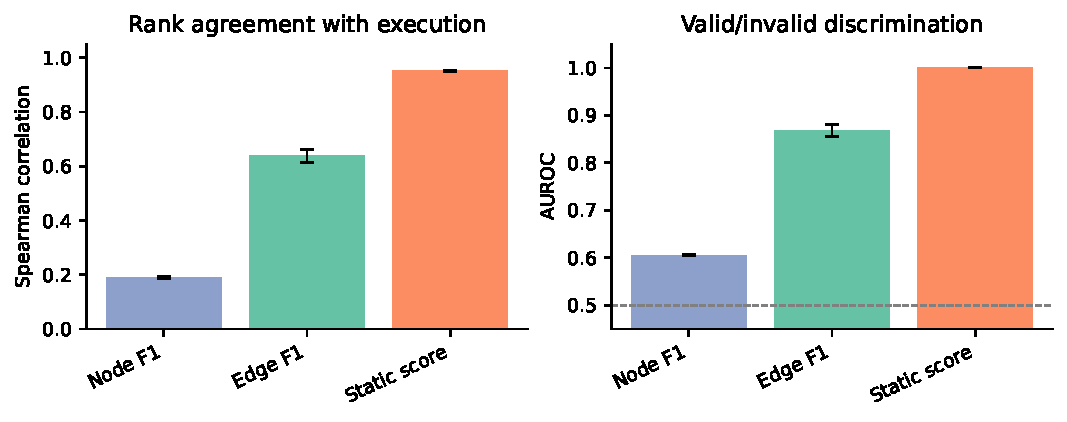
\includegraphics[width=\linewidth]{figures/metric_comparison.pdf}
\caption{Agreement with verified execution on the controlled benchmark.
Error bars show 95\% intervals from 2,000 task-cluster resamples, with all seven
variants of each task kept together. The intervals describe repeated sampling
from these 50 symbolic tasks, not uncertainty over unseen domains or failure
modes.}
\label{fig:metrics}
\end{figure}

Strict reference matching rejected 130 of the 150 valid non-reference plans,
or 86.7\%. Every equivalent-tool plan executed successfully, even though mean
node F1 fell to 0.793 and mean edge F1 to 0.693. The reverse pattern appeared
for dependency reversal: node F1 stayed at 1.00, yet every plan failed. Edge F1
was more informative than node F1 about dependencies, but harmless structural
changes still moved the score substantially.

Figure~\ref{fig:variants} shows the two error directions side by side. Equivalent-tool
plans obtain the same structural means as wrong-tool plans (node F1 0.793,
edge F1 0.693), although all former plans succeed and all latter plans fail.
The metrics cannot tell the two groups apart because they see labels and edges,
not the contracts behind the tools. Reversed-dependency plans expose the other
side of the problem. Their mean node F1 remains 1.00 and edge F1 is 0.760, but
the imposed ordering causes every plan to fail. Missing-producer plans likewise
retain a fairly high mean node F1 of 0.884. For AQ1, these are the clearest
disagreements: semantic substitution hurts similarity without hurting validity,
whereas the wrong dependency direction can preserve similarity and break
execution.

\begin{figure}[t]
\centering
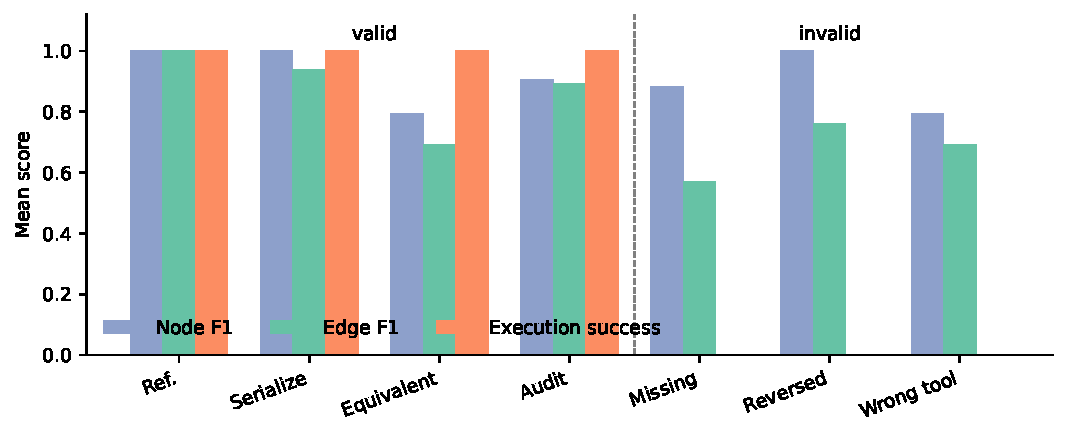
\includegraphics[width=\linewidth]{figures/variant_analysis.pdf}
\caption{Mean structural scores and execution success by controlled variant.
Each bar summarizes 50 plans. The first four variants are valid.}
\label{fig:variants}
\end{figure}

The static score separates all designed valid and invalid variants in this
benchmark without calling the executor. This is still an internal construct
check, not evidence of open-world generalization: the catalog schemas and
candidate transformations are generated from the same symbolic contracts.
The post-execution full score is not included in Table~1 because correlating a
score that contains outcome success with outcome success would be circular.

\begin{table}[t]
\centering
\caption{Static-component ablation on the controlled benchmark.}
\label{tab:ablation}
\begin{tabular}{lcc}
\toprule
Static evaluator & Spearman $\rho$ & AUROC \\
\midrule
Dependency validity only & 0.951 & 1.000 \\
Schema executability only & 0.470 & 0.667 \\
Combined static score & 0.951 & 1.000 \\
\bottomrule
\end{tabular}
\end{table}

Table~\ref{tab:ablation} shows that dependency validity, rather than schema
membership, drives discrimination in the current construction. Adding static
executability detects unavailable tools but does not improve aggregate AUROC.
This negative ablation result further limits the strength of the method claim.
The weight sweep confirms the same limitation: every nonzero dependency weight
from 0.05 to 1.00 yields AUROC 1.00 and nearly identical rank correlation,
whereas executability alone yields AUROC 0.667. The apparent robustness is thus
a plateau created by the benchmark design, not evidence that equal weighting is
optimal. New independently designed failure modes are needed to identify useful
component weights.

In the Qwen3-8B pipeline check, all 30 outputs parsed as JSON and all executed
successfully; mean latency was 3.96 seconds. Each generated plan exactly matched
its reference graph. This confirms that generation and evaluation work end to
end, but it tells us nothing about how the metrics behave when plans differ.

\begin{table}[t]
\centering
\caption{Local-model pipeline check (10 tasks, three seeds). The fixed output
budget was 1,200 tokens per plan.}
\label{tab:models}
\begin{tabular}{lrrrr}
\toprule
Model & Plans & Parse rate & Success rate & Mean latency (s) \\
\midrule
Qwen3-8B & 30 & 1.00 & 1.00 & 3.96 \\
Qwen3-4B & 30 & 0.20 & 0.00 & 12.17 \\
\bottomrule
\end{tabular}
\end{table}

Qwen3-4B often produced long reasoning traces and exhausted the fixed
budget before completing the requested JSON. Only six outputs were parseable;
none formed an executable, goal-completing plan. Under the stated protocol,
that is a genuine end-to-end failure. It is not, however, a clean estimate of
the intrinsic gap between 4B and 8B models. A larger budget, another reasoning
mode, grammar-constrained decoding, or retries after invalid JSON could all
change the result. We retain the uncorrected outputs because format compliance
is itself part of agent reliability, and post-hoc repair would amount to a
different pipeline.

\subsection{Natural Plans on External Benchmarks}
Across 360 generations, 358 parsed into valid DAGs (99.4\%). Mean node F1 was
0.564 and mean edge F1 was 0.258; fuzzy node matching raised the node score to
0.688. The three runs for a task were relatively stable (mean node-set Jaccard
0.941 and edge-set Jaccard 0.945), so the low agreement cannot be dismissed as
random formatting noise alone.

\begin{table}[t]
\centering
\caption{Reference agreement for naturally generated external plans. These
scores are descriptive and are not execution-success rates.}
\label{tab:externalplans}
\begin{tabular}{lrrrr}
\toprule
Benchmark & Plans & Parse & Node F1 & Edge F1 \\
\midrule
WorFBench & 180 & 98.9\% & 0.171 & 0.032 \\
TaskBench & 180 & 100.0\% & 0.957 & 0.483 \\
\midrule
Overall & 360 & 99.4\% & 0.564 & 0.258 \\
\bottomrule
\end{tabular}
\end{table}

Agreement depended strongly on benchmark representation. Within WorFBench,
mean node F1 ranged from 0 on WebShop to 0.495 on WikiHow, although catalog
validity remained 96.7--100\%. Within TaskBench, node F1 ranged from 0.940 to
0.983 while edge F1 ranged from 0.432 to 0.568. These figures do not establish
that the generated plans are correct. They do show that the same model and
prompt can look radically different under reference labels and graph
conventions, reinforcing the need for execution or independent semantic
judgment before treating F1 as validity.

The non-Qwen sensitivity run confirms substantial model dependence. Among 120
Gemma3-1B plans, 97.5\% parsed, but only 58.3\% formed valid DAGs; mean node F1
was 0.187, mean edge F1 0.002, and catalog validity 0.314. On the same 120 tasks,
Qwen3-8B run 1 had 100\% valid DAGs, node F1 0.564, edge F1 0.259, and catalog
validity 0.996. Paired Qwen-minus-Gemma differences were 0.417 for DAG validity
(95\% task-bootstrap CI $[0.333,0.508]$), 0.377 for node F1
($[0.298,0.455]$), 0.257 for edge F1 ($[0.188,0.328]$), and 0.682 for catalog
validity ($[0.604,0.759]$). These differences show that pipeline reliability
does not transfer automatically across model choices; they do not isolate
architecture or scale as the cause.

\subsection{AI-Assisted Blind Annotation}
The two raw AI annotators agreed on 93 of 120 overall validity labels (77.5\%).
Cohen's $\kappa$ was 0.478 (95\% task-bootstrap CI $[0.304,0.636]$), which is
only moderate agreement. Of the 27 disagreements, Qwen3-4B called 11 plans
valid that Qwen3-8B called invalid, while the reverse pattern did not occur.
This asymmetry was concentrated in plans requiring state tracking or missing
actions, especially ALFWorld.

\begin{table}[t]
\centering
\caption{Agreement between two blind AI-assisted annotation runs on 120
natural plans. These values measure model-annotation repeatability, not human
inter-annotator reliability.}
\label{tab:aiagreement}
\begin{tabular}{lrrr}
\toprule
Field & Agreement & $\kappa$ & 95\% CI \\
\midrule
Overall validity & 0.775 & 0.478 & [0.304, 0.636] \\
Tool selection & 0.758 & 0.412 & [0.240, 0.572] \\
Dependency validity & 0.742 & 0.246 & [0.057, 0.423] \\
Executability & 0.742 & 0.372 & [0.211, 0.527] \\
Goal completion & 0.642 & 0.222 & [0.128, 0.310] \\
Alternative validity & 0.567 & 0.141 & [-0.009, 0.296] \\
Primary error type & 0.742 & 0.412 & [0.249, 0.560] \\
\bottomrule
\end{tabular}
\end{table}

The post-audit analysis labels contain 92 valid, 18 partially valid, and 10
invalid plans. We treat those counts as a diagnostic artifact, not ground
truth. In a pooled sensitivity analysis, node F1 correlates more strongly with
the audited ordinal label than edge F1 ($\rho=0.496$, task-bootstrap 95\% CI
$[0.363,0.612]$, versus $0.231$, $[0.083,0.356]$). This apparent signal does
not survive control for benchmark subset: within-subset centered correlations
are $-0.030$ for node F1 and $-0.095$ for edge F1. Fuzzy node F1 and a simple
node--edge overlap baseline behave similarly ($-0.020$ and $-0.083$), while
catalog validity is essentially uninformative ($0.040$).

The label distribution explains the reversal. All 20 TaskBench multimedia
plans are labeled valid, 38 of the other 40 TaskBench plans are valid, and 8 of
the 10 invalid labels occur in WorFBench ALFWorld. Several subset-level AUROCs
are undefined because a subset contains only one class; where both classes are
present, node-F1 AUROC ranges from 0.406 on WikiHow to 0.545 on ALFWorld. A
diagnostic pair makes the problem concrete: \texttt{worf\_webshop\_266} is
labeled valid despite node and edge F1 of zero, whereas
\texttt{worf\_wikihow\_14} is labeled invalid with node F1 0.667. These are
model-assisted judgments rather than definitive counterexamples, but they show
why pooled correlation cannot support a metric-validity claim. More
importantly, the modest $\kappa$ shows that replacing a single reference with a
single model judge does not solve multiplicity; it changes the source of
evaluator uncertainty.

\subsection{Completed Paired Blind Annotation}
Both returned workbooks contained 120 unique annotation IDs in identical task
order, with complete categorical fields and rationales. The passes agreed on
91 of 120 overall-validity judgments (75.8\%), giving Cohen's
$\kappa=0.536$ (95\% paired task-bootstrap CI $[0.409,0.667]$). Agreement was
strongest for executability ($\kappa=0.768$) and tool selection
($\kappa=0.722$), but dependency validity remained notably less stable
($\kappa=0.437$). All five core fields agreed simultaneously for 91 plans.
Across all seven fields, 29 plans contained at least one disagreement and are
covered by the separate adjudication record. It contains exactly these 29 IDs,
no duplicates or missing required fields, and no out-of-codebook final values.
Combining its decisions with the 91 agreed rows produces a complete 120-plan
analysis layer.

\begin{table}[t]
\centering
\caption{Agreement between the two completed blind annotation passes on 120
natural plans. The workbooks are complete, but file provenance alone does not
verify distinct or independent human raters.}
\label{tab:pairedagreement}
\begin{tabular}{lrrr}
\toprule
Field & Agreement & $\kappa$ & 95\% CI \\
\midrule
Overall validity & 0.758 & 0.536 & [0.409, 0.667] \\
Tool selection & 0.892 & 0.722 & [0.606, 0.845] \\
Dependency validity & 0.867 & 0.437 & [0.214, 0.653] \\
Executability & 0.908 & 0.768 & [0.640, 0.881] \\
Goal completion & 0.842 & 0.659 & [0.539, 0.783] \\
Alternative validity & 0.842 & 0.652 & [0.511, 0.784] \\
Primary error type & 0.833 & 0.691 & [0.555, 0.815] \\
\bottomrule
\end{tabular}
\end{table}

The agreement result materially improves coverage over the earlier AI-only
audit and identifies which judgments are reproducible. Pass A used
``Partially valid'' 32 times and pass B only seven times, so the moderate
overall $\kappa$ is substantively important rather than a formatting artifact.
After adjudication, the final distribution is 72 valid, 21 partially valid,
and 27 invalid. The adjudicated analysis in Table~\ref{tab:adjudicatedmetrics}
does not rescue reference matching: node F1 separates valid from other plans
only slightly better than chance, and edge F1 does worse than chance. The
positive pooled node association also falls from $\rho=0.240$ to $0.084$ after
within-subset centering.

\begin{table}[t]
\centering
\caption{Association with the final adjudicated overall-validity labels on 120
natural plans. AUROC treats valid as positive and partial/invalid as negative;
confidence intervals use 2,000 task bootstrap resamples.}
\label{tab:adjudicatedmetrics}
\begin{tabular}{lrrr}
\toprule
Evaluator & Spearman $\rho$ (95\% CI) & AUROC (95\% CI) & Centered $\rho$ \\
\midrule
Node F1 & 0.240 [0.051, 0.419] & 0.572 [0.473, 0.672] & 0.084 \\
Edge F1 & 0.030 [$-$0.151, 0.195] & 0.458 [0.362, 0.551] & $-$0.140 \\
Fuzzy node F1 & 0.231 [0.044, 0.416] & 0.572 [0.471, 0.675] & 0.196 \\
Node--edge average & 0.192 [0.005, 0.368] & 0.540 [0.433, 0.646] & $-$0.095 \\
Catalog validity & $-$0.073 [$-$0.141, $-$0.062] & 0.493 [0.477, 0.500] & $-$0.002 \\
\bottomrule
\end{tabular}
\end{table}

These numbers are evidence against single-reference matching, not a calibrated
estimate of a human population parameter. The adjudication file names one
adjudicator and supplies dated rationales, but the artifact itself cannot prove
who performed the work or whether that person was independent.

\subsection{Typed-Contract Results}
All 40 TaskBench Multimedia and Hugging Face run-1 plans were valid DAGs and
used catalog-listed tool names, so catalog validity was constant and
uninformative. Mean edge-type compatibility was 0.947. As shown in
Table~\ref{tab:typedcontracts}, the resulting diagnostic has AUROC 0.631, but
its interval includes chance because only nine plans are partial or invalid.
Because graph and catalog validity are both one for every plan, the composite
has the same ranking as edge compatibility. The experiment therefore provides
an external, reference-free check that typed contracts carry some signal, while
also demonstrating that schema and type checks alone do not establish plan
validity.

\begin{table}[t]
\centering
\caption{Reference-free typed-contract diagnostic on 40 TaskBench plans with
benchmark-supplied tool input/output types. AUROC treats valid as positive.}
\label{tab:typedcontracts}
\begin{tabular}{lcc}
\toprule
Evaluator & Spearman $\rho$ (95\% CI) & AUROC (95\% CI) \\
\midrule
Catalog validity & 0.000 [0.000, 0.000] & 0.500 [0.500, 0.500] \\
Edge-type compatibility & 0.365 [$-$0.095, 0.712] & 0.631 [0.470, 0.809] \\
Typed-contract composite & 0.365 [$-$0.095, 0.712] & 0.631 [0.470, 0.809] \\
\bottomrule
\end{tabular}
\end{table}

\subsection{External ALFWorld Execution}
The agent completed 35 of 120 distinct ALFWorld tasks, for a success rate of
29.2\% (Wilson 95\% CI $[21.8,37.8]$). All 4,915 selected actions were listed
as admissible by the environment, but the median episode still reached the
50-step limit. Legal local actions therefore did not guarantee successful
long-horizon execution.

\begin{table}[t]
\centering
\caption{Qwen3-8B execution on ALFWorld \texttt{valid\_unseen}. Intervals are
95\% Wilson intervals for the success proportion.}
\label{tab:alfworld}
\begin{tabular}{lrrr}
\toprule
Task type & Success & Rate & 95\% CI \\
\midrule
Pick and place & 9/22 & 40.9\% & [23.3, 61.3] \\
Look under light & 12/18 & 66.7\% & [43.7, 83.7] \\
Clean then place & 5/21 & 23.8\% & [10.6, 45.1] \\
Heat then place & 0/21 & 0.0\% & [0.0, 15.5] \\
Cool then place & 2/21 & 9.5\% & [2.7, 28.9] \\
Place two objects & 7/17 & 41.2\% & [21.6, 64.0] \\
\midrule
Overall & 35/120 & 29.2\% & [21.8, 37.8] \\
\bottomrule
\end{tabular}
\end{table}

Performance was strongly task-dependent. Looking at an object under a light
was easiest, while no heat-then-place task finished within the budget. The
result does not validate the controlled static score on ALFWorld because that
environment exposes commands rather than our symbolic plan contracts. It does,
however, add independent evidence that execution outcome reveals failures that
command admissibility alone misses.

The frozen-plan comparison exposes a stricter failure mode. None of the 30
single-shot plans succeeded (Wilson 95\% CI $[0.0,11.4]$), whereas the matched
reactive runs succeeded on 8/30 tasks (26.7\%, $[14.2,44.4]$). All eight
discordant pairs favored the reactive policy, giving $p=0.0078$ under the
two-sided exact McNemar test. Nevertheless, the frozen plans had mean schema
validity 0.995, mean abstract dependency validity 0.872, and a mean composite
pre-execution score of 0.934. Their commands were admissible at the moment of
execution 72.8\% of the time. The pre-execution score correlated with this
local admissibility rate ($\rho=0.578$), but success discrimination is undefined
because every frozen plan failed.
Gemma3-1B also completed 0/30, but generated much weaker plans: mean length
3.77, parse success 93.3\%, contemporaneous admissibility 7.9\%, and mean
pre-execution score 0.532. Thus its failure cannot be attributed cleanly to
open-loop execution; output quality is already a dominant limitation.

\begin{table}[t]
\centering
\caption{Matched ALFWorld execution with and without observation-conditioned
replanning. The frozen score averages schema and abstract-dependency validity.}
\label{tab:frozen}
\begin{tabular}{lrrr}
\toprule
Protocol & Success & 95\% Wilson CI & Pre-score \\
\midrule
Frozen single-shot & 0/30 & [0.0, 11.4] & 0.934 \\
Frozen Gemma3-1B & 0/30 & [0.0, 11.4] & 0.532 \\
Reactive matched & 8/30 & [14.2, 44.4] & -- \\
\bottomrule
\end{tabular}
\end{table}

This result is not evidence that frozen planning is universally impossible.
The initial state hides object locations, so a fixed command sequence cannot
condition later search on observations. Rather, it falsifies a stronger and
tempting interpretation of our controlled result: high static contract scores
alone do not certify task success in a partially observable environment.
Execution-grounded evaluation must represent observation-contingent branches
or explicitly scope its claim to fully specified workflows.

\subsection{Topology and Error Analysis}
Every topology contains 70 candidates with the same four-valid/three-invalid
mix, which fixes the execution success rate at $4/7=0.571$. Edge F1 still
changes markedly: from 0.673 for the diamond to 0.878 for the double diamond;
chain-4, fork--join, and chain-6 score 0.765, 0.783, and 0.866. In other words,
an absolute structural score partly reflects graph size and density even when
the rate of valid plans does not change. A single edge-F1 threshold may
therefore treat topologies with identical failure rates quite differently.
ExecPlanEval instead asks whether the dependencies required by the actual tool
contracts are supported.

None of the 150 invalid controlled plans passes strict matching. That precision
comes at a steep cost: 130 valid alternatives are rejected too. Strict equality
is not useless; it identifies the annotated realization very accurately. It is
just too narrow to serve as the complete definition of plan correctness. This
answers AQ1 without implying that reference graphs should be discarded. They
remain valuable for diagnosis, supervision, and reproducible comparison when
paired with operational checks.

\subsection{Symbolic Pilot Study}
Before running the full benchmark, we checked the core experimental logic in a
small deterministic symbolic environment. The pilot contains 10 task templates
from distinct domains and 60 candidate plans. For every reference plan, we
constructed three valid alternatives (serialization of independent steps,
equivalent-tool substitution, and insertion of a harmless audit step) and two
invalid perturbations (removal of a required branch and reversal of a required
dependency). The executor agreed with the designed validity label on all 60
candidates. Table~\ref{tab:pilot} reports the verified pilot results.

\begin{table}[t]
\centering
\caption{Verified results from the 10-task symbolic pilot. These figures
validate the pipeline but are not evidence for real-world generalization.}
\label{tab:pilot}
\begin{tabular}{lccc}
\toprule
Plan variant & Success rate & Node F1 & Edge F1 \\
\midrule
Reference & 1.00 & 1.00 & 1.00 \\
Valid serialization & 1.00 & 1.00 & 0.86 \\
Valid equivalent tool & 1.00 & 0.75 & 0.67 \\
Valid redundant audit & 1.00 & 0.89 & 0.86 \\
Invalid missing branch & 0.00 & 0.86 & 0.80 \\
Invalid reversed dependency & 0.00 & 1.00 & 0.67 \\
\bottomrule
\end{tabular}
\end{table}

The pilot reveals two diagnostic cases that motivate the full study. First,
structural difference does not necessarily imply operational failure. Replacing
one tool with a symbolically equivalent alternative reduced mean node F1 to
0.75 and edge F1 to 0.67, yet the success rate remained 1.00. Second, choosing
the right nodes is not enough: plans with a reversed dependency retained a node
F1 of 1.00 but all failed during execution. Because the tasks and perturbations
are synthetic and deterministic, we draw no conclusions about naturally
generated agent plans from this pilot alone.

As an implementation check, node F1 achieved an AUROC of 0.50 for separating
valid from invalid pilot plans, and edge F1 achieved 0.8125. The static
ExecPlanEval variant achieved an AUROC of 1.00 and a Spearman correlation of
0.98 with execution success without invoking the executor. The post-execution
full score is not evaluated as a predictor because it directly contains the
outcome label. These results are
expected to favor the contract-aware diagnostic: the pilot was deliberately generated
from the same explicit precondition/effect semantics used by the evaluator.
They therefore establish code-level construct validity only. The external
experiments below add naturally generated plans, unseen benchmark tasks, and
live simulator execution, but validity labels produced independently of the
evaluator remain necessary for a broader semantic claim.

\section{Discussion}
\subsection{What the Controlled Evidence Establishes}
Under exact tool contracts, the experiment establishes a fairly basic but
important existence result: a single gold graph can disagree systematically
with executable validity, even when annotation and execution are noise-free.
The 86.7\% rejection rate is not a prevalence estimate for deployed agents. It
is a design-dependent consequence of applying strict matching to a
balanced collection with three deliberately selected kinds of valid
alternatives. For the same reason, ExecPlanEval's perfect AUROC is best viewed
as an internal check that evaluator and executor implement the same
precondition/effect semantics. Our claim is comparative and deliberately
bounded. In this environment, operational semantics recover distinctions that
label-only graph similarity cannot represent.

The controlled part of AQ2 needs the same qualification. Node F1 has weak rank agreement
($\rho=0.188$), edge F1 is clearly stronger ($\rho=0.638$), and the
static score is strongest ($\rho=0.951$). We do not expect these exact
magnitudes to transfer unchanged to natural tasks. What the comparison does
show is that dependency information matters, and that checking a dependency
against tool semantics can tell us more than asking whether it resembles an
edge in the reference.

\subsection{When Reference Matching Remains Appropriate}
Reference matching remains the right choice when tools have unique identities,
workflows are legally or procedurally fixed, and the annotation defines a
required process rather than one possible route to an outcome. A medical
approval workflow, for example, may prescribe an order even when another order
would produce the same database state. In that setting, conformance is part of
the goal and should be encoded as a hard constraint. ExecPlanEval does not
replace process compliance. It separates compliance, executability, and
outcome, allowing a benchmark to state plainly which notion it evaluates.

\subsection{What the External Evidence Adds}
The external studies address two weaknesses of the controlled construction,
but each supports a different level of claim.
First, the TaskBench and WorFBench sample uses natural instructions and plans that
were not created by applying our own perturbation rules. Its large
between-benchmark F1 differences show that representation choice materially
affects structural scores. Second, ALFWorld supplies environment transitions
and terminal rewards rather than labels generated by ExecPlanEval. The 100\%
admissible-action rate alongside only 29.2\% task success demonstrates a gap
between local command validity and completed long-horizon behavior. Third, the
AI-assisted blind study exposes evaluator instability directly: dependency and
goal-completion judgments obtain $\kappa$ values of only 0.246 and 0.222.
Fourth, the completed paired blind passes show higher agreement on the same
rubric; dependency validity is again the least reliable core component
($\kappa=0.437$). The subsequent adjudication resolves all 29 disagreement
cases and still leaves node- and edge-based reference matching near chance for
binary validity. Fifth, the typed-contract diagnostic avoids the gold graph and
uses benchmark-authored type schemas. Its AUROC of 0.631 is directionally
encouraging but imprecise, and the constant catalog score shows that type/schema
validity alone is insufficient.
The within-subset analysis adds a stronger warning: the positive pooled
association between node F1 and AI-assisted validity is almost entirely a
between-benchmark artifact. None of the structural baselines shows positive
within-subset rank agreement in this sample.

None of these checks proves that ExecPlanEval generalizes unchanged. The
natural-plan sample now has two complete paired annotation passes and a
complete adjudicated analysis layer, but file provenance does not independently
verify distinct rater identities, independence, or adjudicator identity. The two AI
annotators are neither model-family-independent nor generator-independent.
ALFWorld does not
expose the symbolic contracts required to compute every ExecPlanEval component.
Only two TaskBench subsets expose enough typed metadata for the restricted
contract diagnostic, and even these lack argument bindings, missing-edge
verifiers, and execution outcomes. We therefore use the external evidence to test failure modes and ecological
plausibility, not to claim an externally measured AUROC for the diagnostic.
The resulting evidence hierarchy is therefore explicit: the controlled
benchmark supports causal statements about known plan perturbations; the
natural-plan sample supports descriptive statements about representation
sensitivity; the dual AI annotation supports model-judge repeatability; the
paired blind passes and adjudication support rubric feasibility, agreement
analysis, and a resolved label layer but not a certified human gold standard;
and ALFWorld supports a behavioral sanity
check of long-horizon tool use.

\subsection{Further Open-World Validation}
Moving beyond the present external checks requires four additions. First,
tool equivalence should
be established by held-out contracts or empirical tests, not copied effects.
Second, the identities, relevant expertise, and independence of both original
contributors and the adjudicator should be documented without exposing personal
identifiers in the release. Third, stochastic execution should use repeated
trials and report success probabilities with costs and side effects. Fourth,
tasks and tool families used to design verifiers should be separated from the
test set. Together, these steps would turn the current construct-validation
benchmark into a generalization study and make it possible to calibrate weights
without test leakage.

\section{Reproducibility}
The released artifact contains the 50-task JSON benchmark, every candidate
graph, raw Qwen outputs, per-plan CSV results, aggregate JSON summaries, and
scripts for generation, execution, scoring, bootstrap analysis, and figure
production.
It also contains all 480 natural external plans, static diagnostic scores, the
fixed blind-annotation workbook and codebook, the fixed ALFWorld sampling
manifest, all 120 raw execution
trajectories, episode- and task-type-level CSV files, and the Wilson-interval
summary. The ALFWorld runner validates completed files and resumes without
resampling or overwriting them.
The annotation release additionally contains both raw AI runs, the 27-item
disagreement table, field-level agreement and $\kappa$ values, bootstrap
intervals, and the separate audited analysis labels. Raw labels are immutable;
the audit is stored as another layer rather than silently replacing them.
It also preserves both completed annotation workbooks, normalized JSONL
exports, the raw 29-case adjudication record, the validated 120-case final label
layer, field-level agreement, and fixed-seed bootstrap intervals. Neither pass
is overwritten by the adjudicated layer. The analysis script verifies exact ID
coverage and codebook membership before computing final distributions,
correlations, and AUROC.
It also includes a provenance packet with SHA-256 hashes and separate
declaration templates for Contributors A and B and the adjudicator. These forms
are intentionally marked incomplete: they become evidence only when personally
completed and verified by the respective contributors and a study custodian.
The typed-contract release contains the per-plan scores, benchmark-authored
schema source paths, and fixed-seed analysis output for all 40 eligible plans.
The release also includes the subset-stratified analysis, task-bootstrap
intervals, diagnostic cases, and the complete 21-point weight sweep.
Controlled generation and task-cluster bootstrap sampling use fixed seeds. Assertions test
all 350 designed labels against actual execution; the analogous pilot test
covers all 60 pilot plans. The model study records model identifier, run index,
temperature, latency, raw response, parse error, materialized plan, validation
errors, and failure reason. No API key or proprietary service is needed; the
reported model runs use a local Ollama endpoint.

Reproducing the controlled pipeline involves three stages: generate the
dataset, execute the benchmark, and produce figures from the saved summary.
Keeping these stages separate prevents a plotting or manuscript change from
altering raw results. The local-model result files are named by checkpoint to
avoid accidental overwriting. The data contain no environment-specific
absolute paths, and every number reported in the tables can be recovered from
the corresponding JSON summary.

\section{Limitations and Ethics}
Several limitations matter here. Execution environments cannot capture every
real-world side effect, human judgments of validity may still differ, and any
model-based semantic component can introduce evaluator bias. Tools with
irreversible external effects should not be run directly. More importantly,
our primary benchmark is controlled and symbolic: tool names expose domain and
topology, outcomes are deterministic, and the candidate transformations come
from the same precondition/effect semantics used by the evaluator. This is why
ExecPlanEval attains perfect AUROC, and it is also why that number is not an
estimate of open-world performance. The nominal domains change labels rather
than environment dynamics; they should not be mistaken for independent
real-world domains. Likewise, the task-cluster intervals are conditional
resampling summaries for the 50 generated tasks, not frequentist coverage for a
population of domains or unseen perturbation mechanisms. Their narrowness is
partly a consequence of applying the same seven variant types to every task.
The external metric comparisons are exploratory and no multiplicity-adjusted
hypothesis tests are claimed. The typed-contract analysis covers only 40 plans,
contains nine non-valid labels, and cannot detect absent edges or bad arguments;
its wide interval precludes a superiority claim. The ALFWorld study adds genuine simulator interaction, but
it remains one text environment with two capacity-mismatched models,
deterministic decoding, and a
fixed step budget. The natural-plan sample includes two Qwen3 label sets and
two subsequently completed paired blind workbooks. Qwen3-8B generated the
plans and also served as one AI annotator, creating a clear self-evaluation
risk; the assistant-led audit is not a third independent judge. The paired
workbooks are complete, but their identical batch timestamps and substantial
verbatim rationale overlap mean that the files alone cannot establish distinct
identities or independent work. We therefore report them transparently as
paired annotation passes, not as certified independent human ground truth. The
submitted adjudication layer resolves every categorical disagreement, but its
identifier and date fields likewise cannot authenticate the contributor. A
convincing follow-up still needs provenance documentation, stochastic tool
failures, additional models and environments,
and held-out execution rules.
The frozen-plan test closes the specific separation between pre-generation
and execution, but its all-failure outcome prevents estimating score AUROC and
reveals that the current static checker omits partial observability and
contingent replanning.
The external subsets are also label-imbalanced: some contain no AI-labeled
invalid plan, making subset AUROC undefined. Pooled correlations are therefore
not estimates of individual-plan validity.

The benchmark executes only local symbolic actions and produces no external
side effects. We retain model outputs and configurations for auditability. Any
extension beyond this symbolic setting should sandbox tools, redact sensitive
arguments, and require explicit confirmation before consequential actions.

\section{Conclusion}
No single result in this study justifies replacing reference matching with one
universal score. Instead, the combined evidence identifies where common
evaluation claims break. In the controlled benchmark, valid multiplicity and
dependency errors make graph similarity disagree with execution. In natural
benchmarks, representation and subset choice dominate pooled associations. In
annotation, judgments of dependency and goal completion remain unstable. In
ALFWorld, admissible commands and high static plan scores fail to guarantee
long-horizon success, especially when a frozen plan cannot react to hidden
state.

These findings suggest a layered evaluation practice. Reference matching is
appropriate for canonical or compliance-sensitive workflows; contract checks
are useful when independently authored schemas exist; semantic review is
needed for alternative decompositions; and live execution is necessary when
state, feedback, or side effects determine success. ExecPlanEval illustrates
how these dimensions can be separated, but its perfect controlled AUROC is a
construct check, not evidence of open-world superiority. The typed-contract
diagnostic is suggestive but imprecise, and the frozen execution result exposes
a construct it does not yet model.

The paper's contribution is therefore an audit framework, an evidence
hierarchy, and reproducible failure cases. Stronger claims require authenticated
annotation provenance, capacity-matched model replication, independently
specified contracts and verifiers, and additional execution environments.
Until those conditions are met, evaluation papers should report explicitly
which notion of correctness they measure and avoid treating a single gold graph
as interchangeable with plan validity.

\appendix
\section{Candidate Transformations}
For each task, the reference graph is copied before transformation. The
serialization variant adds an edge only between nodes for which no path exists
in either direction. Equivalent substitution replaces one tool with a catalog
entry having the same precondition and effect sets. The audit variant appends
a node after a terminal producer without changing the required goal. Invalid
missing-producer and reversed-dependency variants alter one causal relation;
wrong-tool replacement assigns a sentinel precondition that cannot be produced.
The executor rejects cycles. Among currently enabled actions it uses a
lexicographical tie-breaker, which makes repeated runs deterministic without
forcing an action whose preconditions are not yet satisfied.

\section{Model Planning Prompt}
The local model receives the natural-language task, initial predicate set,
required final predicate set, and the available tools with preconditions and
effects. It is asked to return a JSON object containing nodes with exact tool
names and directed dependency edges. The instruction states that an edge means
the target depends on the source, independent calls require no edge, all
goal-relevant calls must be included, and unnecessary calls should be omitted.
The parser extracts at most one JSON object. Unknown tools receive an
unsatisfiable sentinel precondition rather than being mapped to a known tool.

\section{Reporting Checklist}
The main controlled sample contains 50 tasks and 350 plans; the preliminary
pilot contains 10 tasks and 60 plans; each pilot local-model condition contains
30 generations. External validation contains 480 natural plans from 120 tasks
and 120 distinct ALFWorld executions; two AI-assisted annotators and two paired
blind annotation passes each label the fixed run-1 natural plan for all 120
tasks, with 29 paired-pass disagreements resolved in a separate adjudication
layer. Confidence intervals use 2,000 fixed-seed non-parametric bootstrap
resamples over the 50 controlled tasks, keeping all seven variants of each task
together. We report all candidate variants, both successful and
failed model generations, the fixed decoding budget, hardware, and negative
results. The paired annotation files are analyzed without claiming identities
or independence that their metadata cannot verify; no personal data or
external side-effecting tool calls are used.

\bibliographystyle{plain}
\bibliography{references}
\end{document}
